\chapter{Моделирование}
\section{Инструменты моделирования}
Для нахождения позиции оптимального совмещения волноводов, необходимо смоделировать поле волновода, и вычислить интеграл перекрытия, формула которого приведена в главе \ref{coupling}. Перебирая варианты взаимного расположения полей, необходимо найти максимальное значение этого интеграла.

Перебор всех теоретически возможных вариантов занимает длительное время, поэтому стоит его упростить, предполагая единственный максимум у функции. Для оптимизации поиска экстремумов функции используют методы координатного спуска, градиентного (наискорейшего) спуска и симплекс-метод.\cite{numeric} 

Предполагая, что у искомого распределения значений интеграла перекрытия имеется только один максимум, используем метод градиентного спуска, поскольку в этом случае он позволит достичь результата за меньшее число итераций. \cite{mathews}

Итак, нам нужен инструмент, позволяющий считать интегралы, проводить итерации и строить графики. В работе используется язык программирования Python, имеющий все необходимое. 

Для решения наших задач, к Python подключаются следующие внешние библиотеки:
\begin{itemize}
	\item NumPy - пакет функций для базовых операций с матрицами (создание и итерация по ним)
	\item SciPy - пакет математических функций, используется для интегрирования и содержит реализацию алгоритма градиентного спуска
	\item Mathplotlib - для вывода полученных результатов в виде графиков.
\end{itemize}

Кроме того, функция распределения Гаусса, для повышения производительности программы, также была вынесена в отдельный модуль.

\section{Моделирование поперечного смещения}

При поперечном смещении центр выходного поля смещается относительно входного на расстояние $\Delta x$, как показано на рисунке \ref{transverse_movement}. Для исследования коэффициента передачи была написана программа, вычисляющая значения интеграла перекрытия в пределах $x \in [-20, 20]$.
Для моделирования использовались два случая
\begin{itemize}
	\item Два одинаковых цилиндрических волновода с радиусом моды 4~мкм
	\item Два разных цилиндрических волновода с радиусами моды 4~мкм и 7~мкм соответственно
\end{itemize}

\begin{figure}[h!]
		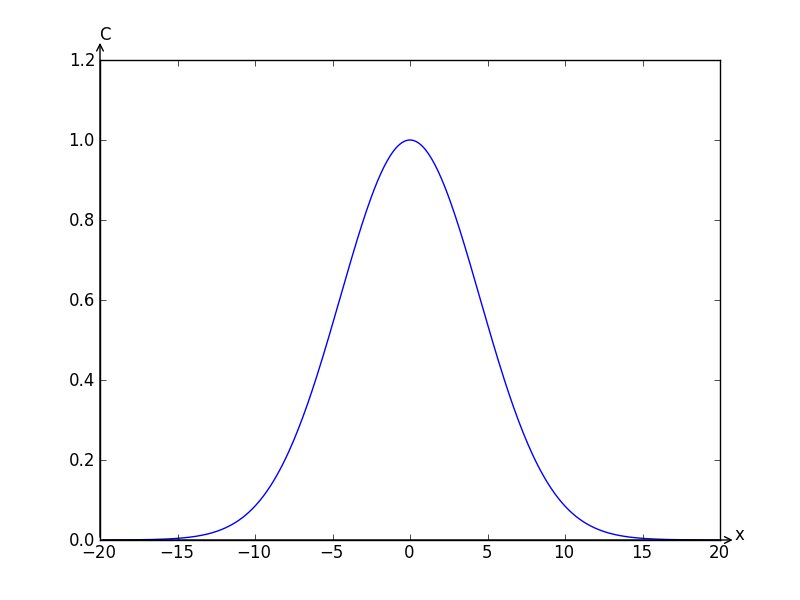
\includegraphics[width=0.5\linewidth]{img/twoCylinders.png}
		\caption{Зависимость коэффициента передачи двух одинаковых волноводов с радиусом моды 4~мкм}
\end{figure}
\begin{figure}[h!]
		\includegraphics[width=0.5\linewidth]{img/twoCylinders2.png}
		\caption{Зависимость коэффициента передачи двух волноводов с радиусами моды 4~мкм и 7~мкм}
		\label{twoCylinders2}
\end{figure}

В ходе моделирования, было обнаружено, что только два одинаковых волновода теоретически позволяют достичь стыковки без потерь. Во втором случае, показанном на рисунке \ref{twoCylinders2} максимальное значение составило 0.862 и это значение будет уменьшаться с ростом разницы в размерах волноводов.

\section{Моделирование продольного смещения}
При продольном смещении необходимо решить задачу нахождения вида пучка на некотором расстоянии от выхода волновода, после чего подставить получившееся распределение в интеграл перекрытия (\ref{coupling}) и определить эффективность передачи.
В моделировании будем использовать планарный волновод, описанный в \ref{strip_field} и цилиндрический с радиусом моды 3~мкм по обеим осям и показателем преломления сердцевины $n$ = 1.47. Длину волны лучей примем $\lambda$ = 1.55~мкм

\begin{figure}[h!]
	\includegraphics[width=0.5\linewidth]{img/longitudinal.png}
	\caption{Коэффициент передачи в зависимости от расстояния между волноводами}
	\label{longitudinal}
\end{figure}

\section{Интерактивная модель}
Для решения основной задачи, то есть поиска точки контакта с максимальным значением коэффициента передачи, была построена отдельная программа.

В ней слева показывается поле в выходном волноводе, а справа - схематическое расположение перекрывающихся полей. Ниже показаны числовые значения рассчитываемых параметров. Изначально программа позиционирует волноводы так, чтобы коэффициент передачи был максимален. Кликами по распределению поля можно виртуально изменять положение выходного волновода относительно входного и изображение будет перестраиваться, показывая новое распределение. Таким образом, можно наблюдать что произойдет при отклонении от точки максимального контакта.

\begin{figure}[h!]
	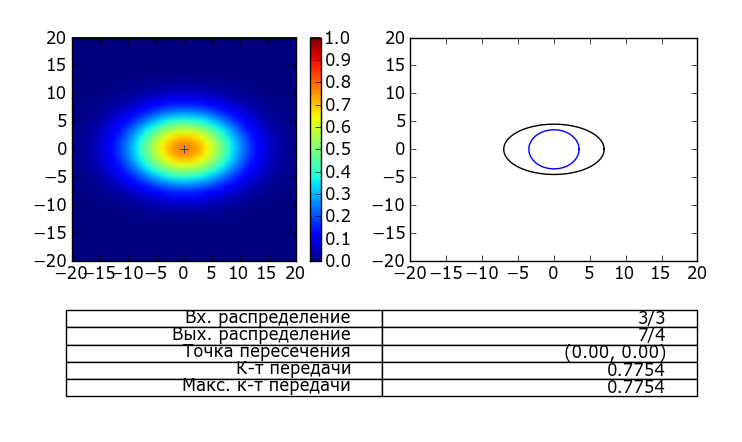
\includegraphics[width=\linewidth]{img/heatmap.png}
	\caption{Общий вид программы}
\end{figure}